% chap6_users.tex
%

\mychapter{User Interactions with Question Answering Systems}
\label{chapter:users}

\noindent

\section{Problem}
\label{section:users:problem}

Most of the research has considered question answering as a one side communication process: a user issues a question and a computer system provides an answer.
Thus, the only input a system receives is the text of the question and the only output is the text of the answer.
This setup is quite limited, because it doesn't provide any means for the user to affect the behavior of a question answering system except by issuing new questions.
Similarly, it doesn't allow QA systems to request any additional information from the user.
However, with the growth of mobile personal assistants and conversational agents the popularity of dialog-based interface increases, which opens up new opportunities for question answering.

TREC complex interactive question answering (ciQA) track, which were run in 2006 and 2007, was designed specifically to motivate research in this area.
In this task participant system could request some input from assessors before submitting the final answer.
However, the setup of the task wasn't exactly based on a dialog between systems and their users.
The most typical approach to the task was to give assessors a set of sentences or passages to judge as relevant/irrelevant and use this feedback to improve the quality of the final answer.
Such scenario is quite problematic to implement in todays personal assistants and chat bots, as they require relatively significant effort and time from users.

In my thesis I'm going to focus on improving the user success solving complex informational tasks in a question answering dialog scenario.
Section~\ref{section:users:approach} describes my prior research on assisting users by providing strategic search hints, designed to help split a complex task into smaller ones that an automatic system will likely handle much better.
And section~\ref{section:users:proposal} proposes additional research to incorporate user feedback into a question answering system in a chat bot scenario.

\section{Approach}
\label{section:users:approach}

%-=-=-=-=-=-=-Search hints begin-=-=-=-=-=-

\subsection{Search Hints for Complex Informational Tasks}
\label{section:users:hints}

Search engines are ubiquitous, and millions of people of varying experience use them on daily basis.
Unfortunately, not all searches are successful.
Bilal and Kirby \cite{Bilal:2002:DSI:637512.637516} reported that about half of the participants of their user study felt frustration when searching.
Xie and Cool \cite{xie2009understanding} demonstrated that most of the time users have problems with formulating and refining search queries.
Besides good retrieval performance, a successful search requires users to possess certain skills.
Search skills can be trained, e.g. Google offers a course\footnote{http://www.powersearchingwithgoogle.com} on improving search efficiency.
Although very useful, such courses are time consuming and detached from real search problems of these particular users.
Displaying search hints is another technique that has both learning effect, and offers immediate assistance to the user in solving her current search task.
Moraveji et al. \cite{Moraveji:2011:MIU:2009916.2009966} demonstrated that hints, suggesting certain search engine functionality, help people find answers more quickly, and the effect is retained after a week without hints.

In this section I explore {\em strategic} search hints, that are designed to guide a user in solving her search problem.
More specifically, we chose the divide-and-conquer strategy, \ie splitting an original difficult question into smaller problems, searching answers to the subtasks and combining them together.
Two sets of strategic hints were manually designed: {\em generic} hints describing the divide-and-conquer strategy in general and {\em task-specific} hints providing a concrete strategy to solve the current search task.
To evaluate the effect of the hints on behavior and search success we conducted a user study with 90 participants.
The results of the user study demonstrate that well-designed task-specific hints can improve search success rate.
In contrast, generic search hints, which were too general and harder to follow, had negative effect on user performance and satisfaction.

\subsubsection{User Study}
\label{section:users:hints:userstudy}

\begin{figure}
\centering
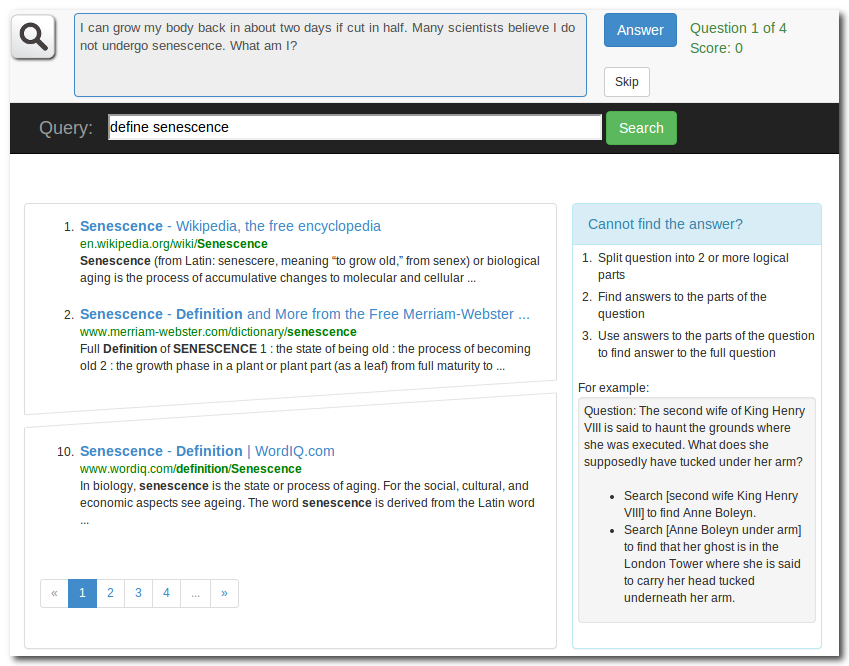
\includegraphics[width=0.75\textwidth]{img/hints_ufindit}
\caption{The interface of the search game used in the study of the effect of strategic search hints on success in solving complex informational tasks}
\label{figure:users:hints:ufindit}
\end{figure}

To estimate the effect of strategic search hints on user behavior we conducted a study in a form of a web search game similar to ``a Google a Day''\footnote{http://www.agoogleaday.com/} and uFindIt \cite{Ageev:2011:FYG:2009916.2009965}. Participants were hired using Amazon Mechanical Turk\footnote{http://www.mturk.com/}. 

The goal of the web search game used in the user study is to find answers to several questions with the provided web search interface (Figure \ref{figure:users:hints:ufindit}). 
Players are instructed not to use any external tools.
The questions are given one by one and since tasks might be too difficult, a chance to skip a question was provided, although users were instructed that effort put into solving a question will be evaluated.
To answer a question each player needs to provide a link to a page containing the answer as well as its text.
The answer is automatically verified and a popup box notifies a player if the answer is incorrect (since the answer can be formulated differently, presence of a keyword was checked).
A player can then continue searching or skip the question when she gives up.
A bonus payment was made to players who answer all questions correctly.
We used Bing Search API\footnote{http://www.bing.com/toolbox/bingsearchapi} as a back-end of the game search interface.
All search results and clicked documents were cached so users asking the same query or clicking the same page got the same results.
At the end of the game a questionnaire was presented asking for feedback on user satisfaction with the game, prior experience and other comments.

\begin{table}[tbh]
\centering
\begin{tabular}{|p{1cm}|p{4.5cm}|p{4.2cm}|p{6.0cm}|} \hline
 & Question & Correct Answer & Specific hints \\ \hline
Task 1 & I can grow body back in about two days if cut in half. Many scientists think I don't undergo senescence. What am I? & Senescence means ``biological aging''. Hydra is considered biologically immortal and regenerates fast. & \parbox[t]{6cm}{
1. Find what is senescence \\
2. Find who does not undergo senescence \\
3. Find who can also regenerate body and choose the one that satisfies both conditions} \\\hline
Task 2 & Of the Romans "group of three" gods in the Archaic Triad, which one did not have a Greek counterpart? & Archaic Triad includes Jupiter, Mars and Quirinus. Among those Quirinus didn't have a Greek counterpart. &
\parbox[t]{6cm}{
1. Find the names of the gods from the Archaic triad\\
2. For each of the gods find a Greek counterpart
}\\ \hline
Task 3 & As George surveyed the ``waterless place'', he unearthed some very important eggs of what animal? & "Gobi" in Mongolian means ``Waterless place''. The first whole dinosaur eggs were discovered there in 1923. & \parbox[t]{6cm}{
1. Find what is the ``waterless place'' mentioned in the question?\\
2. Search for important eggs discovery in this ``waterless place''}\\ \hline
Task 4 & If you were in the basin of the Somme River at summers end in 1918, what language would you have had to speak to understand coded British communications? & Cherokee served as code talkers in the Second Battle of the Somme. & \parbox[t]{6cm}{
1. Find the name of the battle mentioned in the questions\\
2. Search for which coded communications language was used in this battle\\
} \\ \hline
\end{tabular}
\caption{Search tasks used for the study, and specific search hints shown to one of the user groups}
\label{table:users:hints:tasks}
\end{table}

The tasks for the study were borrowed from the ``A Google a Day'' questions archive.
Such questions are factual, not ambiguous and usually hard to find the answer with a single query, which makes them interesting for user assistance research.
We filtered search results to exclude all pages that discuss solutions to ``A Google a Day'' puzzles.
To do this we removed pages that mention a major part of the search question or ``a google a day'' phrase.
To keep users focused throughout the whole game we limited the number of questions to 4.
The tasks are described in Table \ref{table:users:hints:tasks} and were presented to all participants in the same order to ensure comparable learning effects.

The questions have multiple parts and to solve them it is helpful to search for answers to parts of the questions and then combine them.
In one of the previous studies we observed, that most of the users didn't adopt the divide-and-conquer strategy, but kept trying to find the ``right'' query.
We decided to estimate the effect of strategic search hints, suggesting users to adopt the new strategy.

We built 2 sets of strategic hints: \textit{task specific} and \textit{generic}.
Task-specific hints described steps of one of the possible solutions to each question (Table \ref{table:users:hints:tasks}).
Second set contained a single hint, which was shown for all tasks. Generic hint described the divide-and-conquer strategy:\\
\hrule
\begin{enumerate}
\item Split the question into 2 or more logical parts
\item Find answers to the parts of the question
\item Use answers to the parts of the question to find answer to the full question
\end{enumerate}

For example, the question: ``The second wife of King Henry VIII is said to haunt the grounds where she was executed. What does she supposedly have tucked under her arm?''
\begin{enumerate}
\item Search [second wife King Henry VIII] to find Anne Boleyn.
\item Search [Anne Boleyn under arm] to find that her ghost is in the London Tower where she is said to carry her head tucked underneath her arm.
\end{enumerate}
\hrule

To control for the learning effect demonstrated in \cite{Moraveji:2011:MIU:2009916.2009966}, each user was assigned to one of the three groups:
\begin{enumerate}
\item users who didn't get any hints
\item users who got task-specific hints
\item users who got the generic hints
\end{enumerate}


\subsubsection{Results}
\label{section:users:hints:results}

From 199 unique participants, who clicked the HIT on Amazon Mechanical Turk only 90 players finished the game.
We further examined all games manually and filtered out 9 submissions for one of the following reasons: lack of effort (e.g. skipped several tasks after none or a single query) or usage of external resources (e.g. the answer was obtained without submitting any queries or results explored didn't contain the answer).
Furthermore, 10 players from the group which received hints indicated in the survey that they didn't see them, so we filtered out those submissions and finally we had 71 completed games (29 for no hints, 20 for task-specific hints and 22 for generic hints groups).

\textbf{Effects of Search Tips on Performance}.
In order to measure search success rate we looked at the number of questions answered correctly by different groups of users\footnote{Since users were allowed to skip a question we are counting the number of questions that were eventually solved correctly even if a player made some incorrect attempts}.
Figure \ref{figure:users:hints:task_success} shows that success rate is higher for users who saw task-specific hints compared to users who didn't get such assistance.
Surprisingly, having the generic hint decreased the success rate, although users could easily ignore a hint they didn't like.
A possible explanation is: generic hints were harder to follow and users who tried and failed became frustrated and didn't restart their searches.

The plot of average time to answer a question on Figure \ref{figure:users:hints:task_time} doesn't show an improvement for the task-specific hints group, except for the question 1.
Our task-specific hints represent a possible way to solve a problem and there is no guarantee, that it is the fastest one.
It is worth noting, that users from the generic search hint group had slightly higher variance in success time, which can probably be explained by the fact that some users were successful in finding the right way to follow the hint and some other users struggled with it much longer.
Another insight comes from the number of incorrect attempts users made.
Figure \ref{figure:users:hints:incorrect} demonstrates the average number of incorrect answer attempts for all groups of users.
Although the variance is high, there is a tendency for users who saw task-specific hints to make less attempts than both other groups.
This is not in direct correspondence with time spent on the game.
It seems that the users who saw a clear strategy to solve the question were less likely to notice plausible, but incorrect solution.
Moreover, we analyzed texts of incorrect answers, and can conclude that a big part of incorrect submission are due to users trying all possible options they found on the way, even if these options are clearly wrong.


\begin{figure}[h]
\centering
  \begin{subfigure}{0.32\textwidth}
  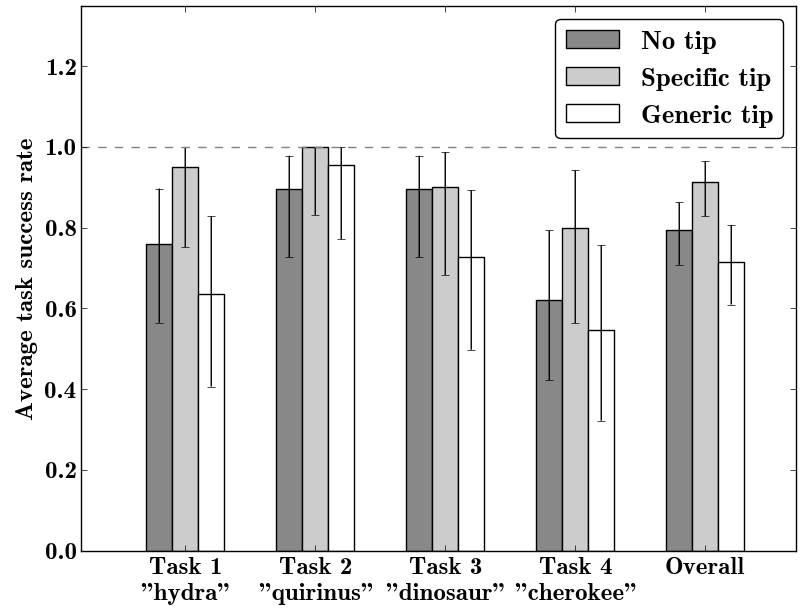
\includegraphics[width=\textwidth]{img/hints_success_per_task}
  \caption{Success rate per task for each group of participants}
  \label{figure:users:hints:task_success}
  \end{subfigure}
  \begin{subfigure}{0.32\textwidth}
  \centering
  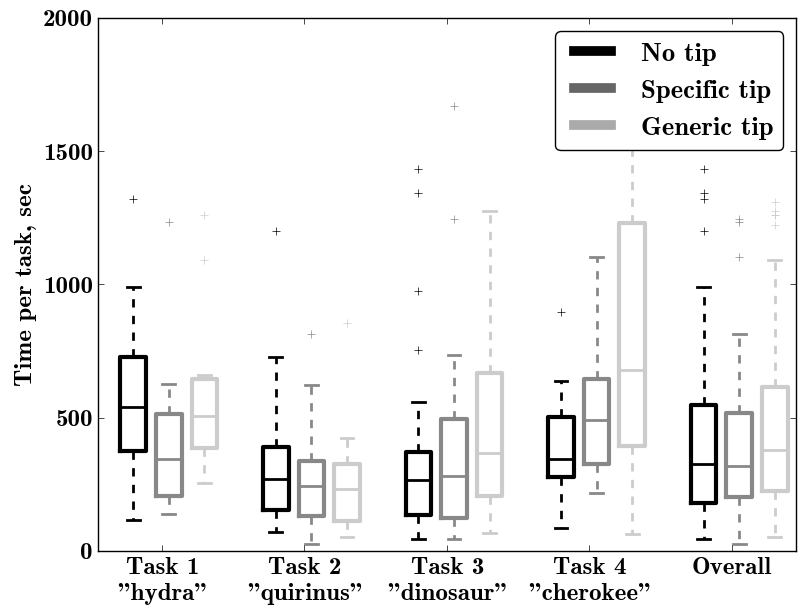
\includegraphics[width=\textwidth]{img/hints_time_per_task}
  \caption{Task completion time for each group of players}
  \label{figure:users:hints:task_time}
  \end{subfigure}
  \begin{subfigure}{0.32\textwidth}
  \centering
  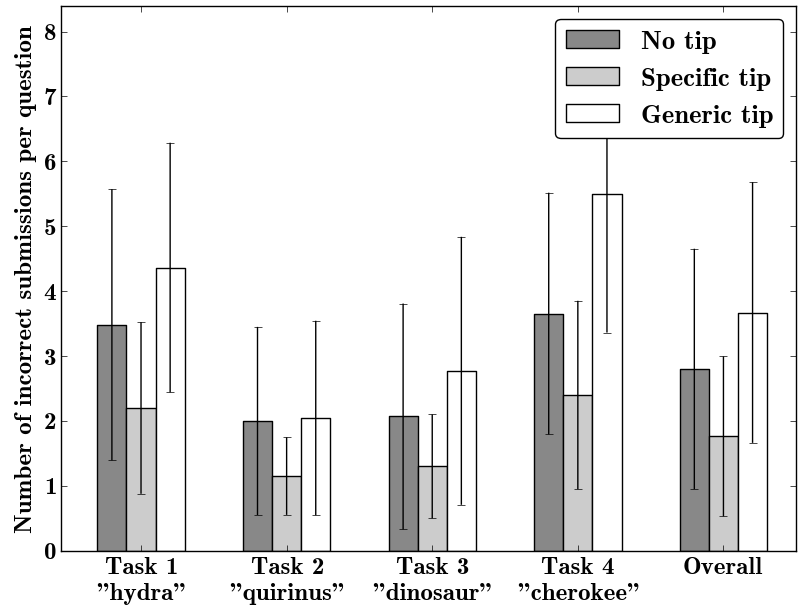
\includegraphics[width=\textwidth]{img/hints_incorrect}
  \caption{The number of incorrect submission attempts per question for all groups of users}
  \label{figure:users:hints:incorrect}
  \end{subfigure}
\caption{Results of the user study on the effectiveness of strategic search tips on search task success rate}
\label{fig:users:hints:results}
\end{figure}

\begin{figure}[h]
\centering
\begin{subfigure}[t]{0.32\textwidth}
	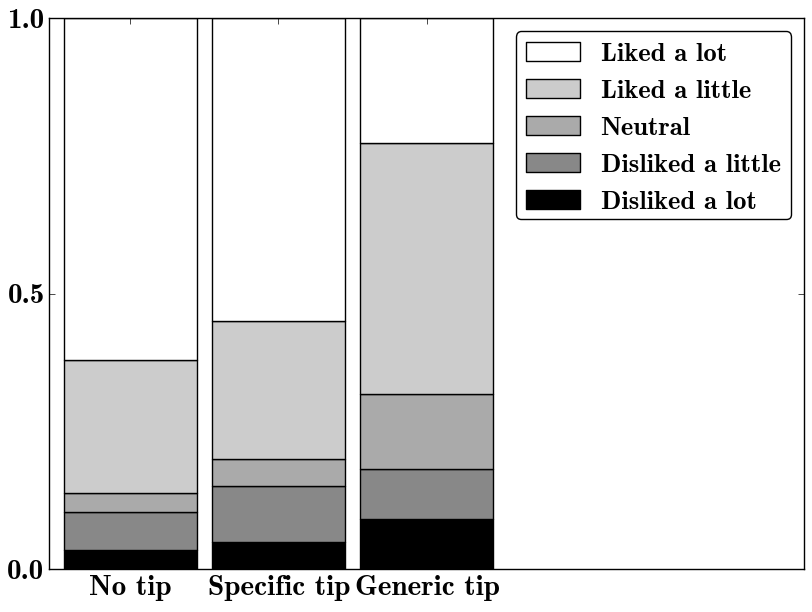
\includegraphics[scale=0.26]{img/hints_liked}
	\caption{How did you like the game?}
    \label{figure:users:hints:survey:liked}
\end{subfigure}
\begin{subfigure}[t]{0.32\textwidth}
	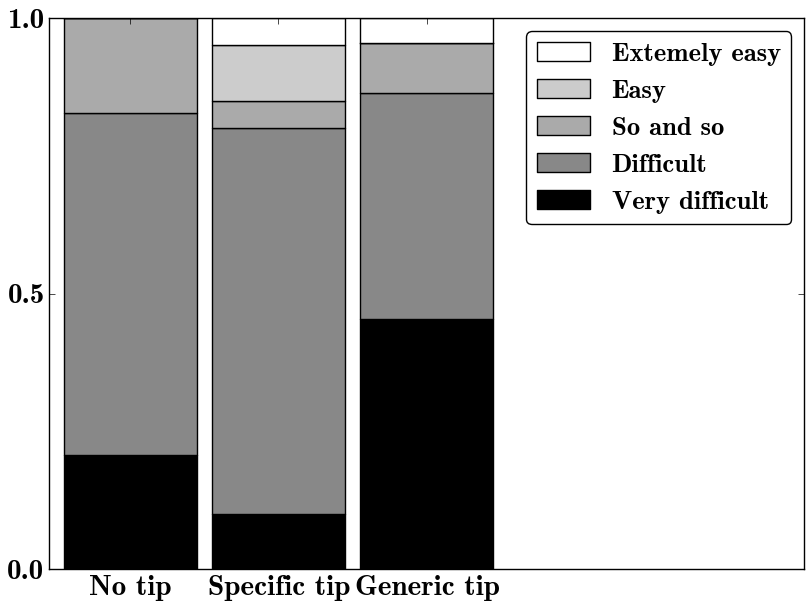
\includegraphics[scale=0.26]{img/hints_difficult}
	\caption{How difficult was the game?}
    \label{figure:users:hints:survey:difficult}
\end{subfigure}
\begin{subfigure}[t]{0.32\textwidth}
	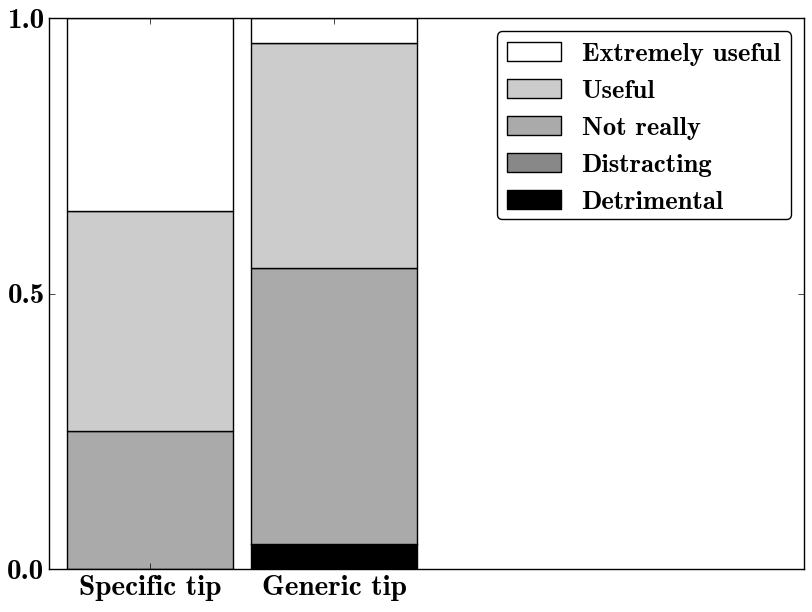
\includegraphics[scale=0.26]{img/hints_useful}
	\caption{Were search hints useful to you?}
    \label{figure:users:hints:survey:useful}
\end{subfigure}
\caption{Proportions of replies to some of the survey question for each group of users}
\label{figure:users:hints:survey}
\end{figure}

We also looked at other search behavior characteristics: number of queries submitted, number of clicks made, average length of the queries. The variance in these characteristics was too high to make any speculations regarding their meaning.

\textbf{Effects of Search Tips on User Experience}.
Finally, we looked at the surveys filled out by each group of users.
Figure \ref{figure:users:hints:survey} presents proportions of different answers to three of the questions: ``How did you like the game?'', ``How difficult was the game?'' and ``Were search hints useful to you?''.
Surprisingly, user satisfaction with the game was lower for users who saw hints during the game and users who didn't get any assistance enjoyed it more.
The replies to the question about game difficulty are in agreement with the success rate: users who saw task-specific hints rated difficulty lower than participants who struggled to find the correct answers.
The game was very difficult on average, however, some participants from the group who received task-specific hints surprisingly rated it as very easy, which suggests that our hints do help users.
This is supported by the answers to the last question on whether hints were helpful (Figure \ref{figure:users:hints:survey:useful}).

To summarize, the results of the conducted user study suggest that specific search hints can be helpful, which is indicated by higher success rate, lower number of incorrect attempts and positive feedback in the end of study survey.
In contrast, generic hints can have negative effect on user experience, which is indicated by lower success rate, increased number of incorrect attempts and higher perceived tasks complexity according to the survey.

\subsubsection{Summary}
\label{section:users:hints:summary}

In this section we studied the effect of strategic search hints on user behavior. 
The conducted user study in a form of a web search game demonstrated the potential of good hints in improving search success rate.
However, to be useful, they should be designed carefully.
Search hints that are too general can be detrimental to search success.
We also find that even searchers who are more effective using specific search hints, feel subjectively less satisfied and engaged than the control group, indicating that search assistance has to be specific and timely if it is to improve the searcher experience.

Even though strategic search hints can improve success rate for complex informational tasks, they represent a rather one-way form of communication, where a system doesn't accept any feedback from the user and doesn't adapt to it.
Hints essentially outsource all the heavy-lifting of decision making to the user, which often makes the experience less enjoyable, as demonstrated by the post-study survey results.
An alternative strategy is to let the system adapt based on the implicit and explicit feedback from the user.
Such a scenario looks even more compelling given a proliferation of personal assistants and chat bots, which makes it easy for users to respond to the user answer with either positive or negative feedback message.

%-=-=-=-=-=-=-Search hints end-=-=-=-=-=-

\section{Proposed Research}
\label{section:users:proposal}

Question answering is one of the major components of modern personal assistants like Apple Siri, Amazon Alexa and Microsoft Cortana.
However, these systems still operate in one sided communication mode, where a user formulates queries and assistant responds with an answer or search results.
In my thesis I propose to incorporate feedback from the user to improve the performance of the question answering system.
To make it more concrete, consider an Example on Figure~\ref{figure:users:proposal:example}.
It's not uncommon for a question answering system to be incorrect.
Web search engines typically decide whether to show direct answers or not based on the confidence in the answer~\cite{yang2015wikiqa}.
However, in a dialog a system needs to provide some kind of response, and why not take a chance and return the top candidate answer.
If the user doesn't like the answer, she can respond accordingly, and this feedback needs to be taken into account by the question answering system, which can then re-rank the candidate answers and provide an alternative response, that will hopefully satisfy the user.

\begin{figure}
\centering
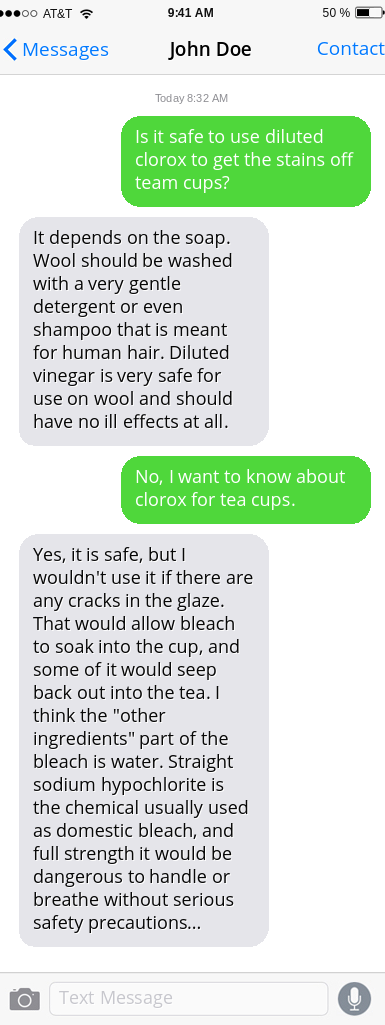
\includegraphics[width=0.3\textwidth]{img/chatbot_example}
\caption{An example of a dialog-based question answering system, that accepts feedback from the user and returns an updated answer}
\label{figure:users:proposal:example}
\end{figure}

Relevance feedback has been studied extensively in the information retrieval community for ad-hoc document retrieval~\cite{salton1997improving,rocchio1971relevance,wang2008study}, but not for question answering.
Thus, I propose to explore the methods for relevance feedback in question answering.

\subsection{Method}
\label{section:users:proposal:method}

In my thesis I propose to focus on both positive and negative relevance feedback for question answering.
A user might give a system a positive feedback if the provided answer was relevant, but either alternative view or additional information is needed.
Alternatively, if an answer is not helpful, a system can take negative feedback to try to generate a good answer.

As a baseline for the experiments I'm planning to take the system I developed for TREC LiveQA shared task, described in Section~\ref{section:non-factoid:liveqa:architecture}, and extend it with the relevance feedback module.
This module will allows the system to adjust and return an alternative answer given either positive or negative feedback.
I'm going to integrate relevance feedback into the system's candidate ranking model.
More specifically, a set of features representing a candidate answer will be extended with various scores, that measure syntactic and semantic similarities between a candidate and positive and negative feedback examples.
This additional set of features will include various vector space, distributed semantics~\cite{kusner2015word} and language model similarity scores~\cite{wang2008study}, as well as some more simple statistics, such as common and missing n-grams, longest common substrings, \etc.
The overall architecture of the proposed system is sketched on Figure~\ref{figure:users:proposal:model}.

There are other alternative stages in the QA pipeline, where we could incorporate the relevance feedback, \eg a system can adjust a set of search queries used to retrieve a set of candidates as done for ad-hoc information retrieval~\cite{rocchio1971relevance}, but I will have to leave this for future work.

\begin{figure}
\centering
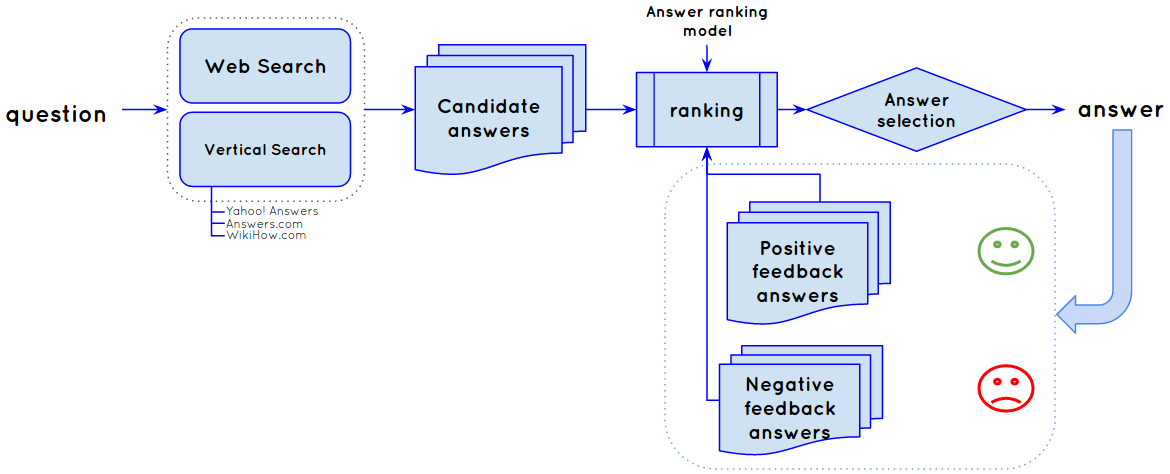
\includegraphics[width=\textwidth]{img/userfeedback_model}
\caption{Architecture of the question answering system, that incorporate positive and negative relevance feedback}
\label{figure:users:proposal:model}
\end{figure}

\subsection{Experimentation}
\label{section:users:proposal:experiments}

To test the system experimentally I propose to reuse the data from TREC LiveQA 2016, which we collected for the crowdsourcing experiment (see Section~\ref{section:crowdsourcing:approach:crqa:experiments}).
As a remainder, during the official run of TREC LiveQA 2016 we collected 1087 questions, issued to our system.
For each question, top 7 generated candidate answers were rated by crowd workers on a scale from 1 (bad) to 4 (excellent).

To test the proposed relevance feedback model I'm proposing to conduct the following simulation experiment.
For each question, top 7 answers will be arranged according to their model score.
Assuming the model returns the top candidate, we collect cases when the top candidate has a low relevance score (\eg $score < 2$), and use these answers as negative feedback.
The goal of the model will be to re-rank the rest of the candidates and return a better answer.
A baseline in this experiment will be a system, that doesn't use the feedback and simply returns the next best answer according to the model score.
Positive relevance feedback experiment will be conducted in a similar way: all answers with good relevance score (\eg from 2 to 3) will be given back to the system as positive feedback with the goal to return another good answer.
This experiment will help us confirm or reject the hypothesis, that it's possible to incorporate relevance feedback for question answering.

To train our ranking model to accept additional answer candidates I will split the original dataset into training and test parts again.
Using the original model I will collect cases with negative and positive feedback as described above, and train the model to retrieve the best possible candidate from the rest of the answers.

However, such simulation experiment won't allow us to test if relevance feedback improves the user experience.
To answer this question we will conduct a user study using either Mechanical Turk or hire some student workers.
We are building a chatbot for Facebook messenger, that will serve as a front-end to our question answering system.
The users will receive a set of questions, e.g. sampled from Yahoo! Answers, and will need to get a satisfactory answer using our chatbot.
All the users will be split into two groups: with and without an option to leave relevance feedback.
The relevance feedback group will be asked to mark each answer as good or bad, after which a new candidate will be provided until the user will decide to stop and declare either fail or success.
The group without relevance feedback will be given an option to receive another answer, which will simply be the next candidate in the original ranked list.
Upon completion of all tasks, the users will complete the questionnaire, where I will ask questions about their experience and satisfaction with the chatbot.
Task success rate and the feedback will help me answer the question if relevance feedback for question answering improves user experience.

\section{Summary}
\label{section:users:summary}

In this chapter I described my prior and proposed research in improving user experience with question answering systems.
Strategic hints, that a system might display to help the user better split the original problem, were shown to be able to improve the success rate, however they need to be designed carefully.
Hints, that are too generic and hard to follow can be distracting and detrimental to the user experience.
However, such hints put all the hard work on the user, who will go through the trial and error process until a system is able to retrieve a good answer.
The second part of the section described the proposed research in engaging in a dialog with the user, and using these interactions to receive relevance feedback, which can be used to refine the answer.
I believe that this feedback is one of the first step, that can lead to deeper understanding of user information needs through dialog.
